\begin{figure}
    \centering
    \caption{Logarithmic Execution time of the Raspberry Pi.}
    \label{fig:log-rpi-execution}
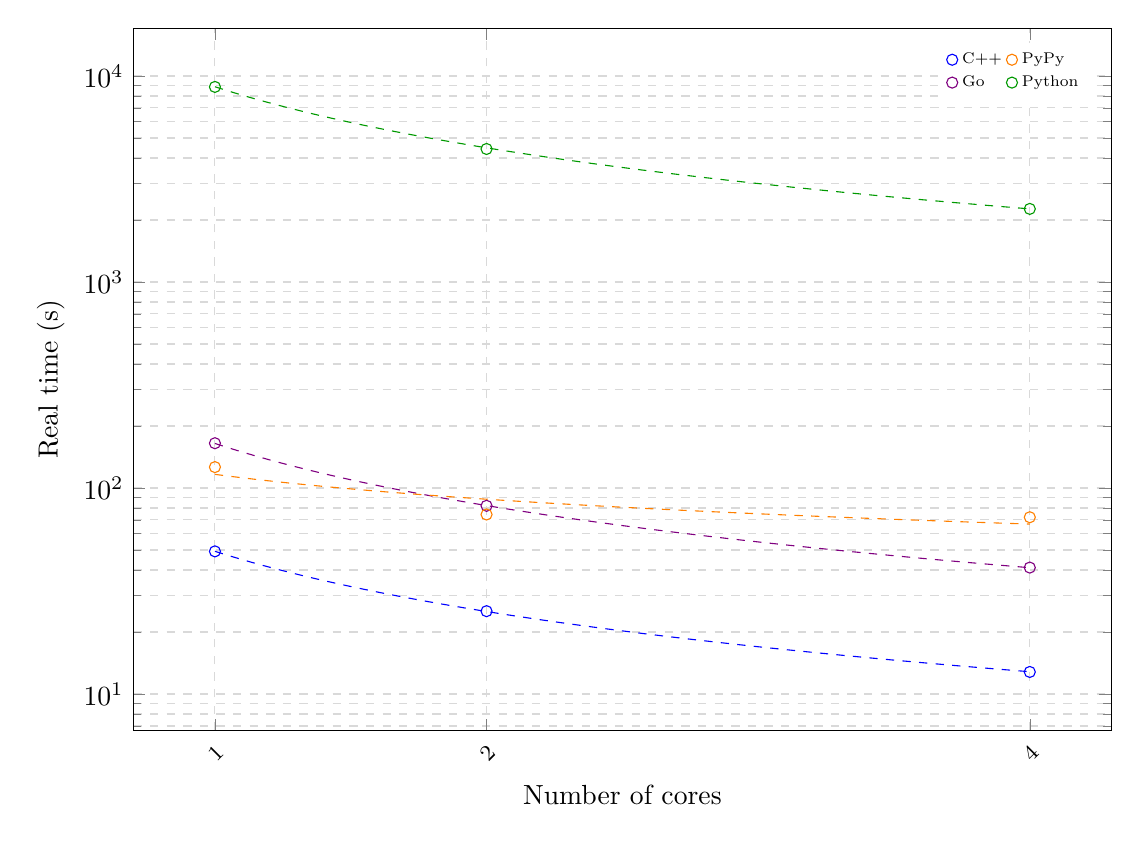
\begin{tikzpicture}
  \begin{semilogyaxis}[
      width=14cm,
      height=10.5cm,
      xlabel={Number of cores},
      ylabel={Real time (s)},
      ymode=log,
      xmode=linear,
      grid=both,
      minor tick num=1,
      grid style={gray!30,dashed},
      xtick={1,2,4},
      x tick label style={
        font=\footnotesize,
        rotate=45,
        anchor=north east
      },
      legend style={
        at={(0.98,0.98)},
        anchor=north east,
        font=\scriptsize,
        nodes={scale=0.8,transform shape},
        draw=none
      },
      legend columns=2,
      transpose legend,
      legend cell align=left,
    ]

    %% C++ %%
    \addplot[
      blue, only marks, mark=o,
      mark options={draw=blue,fill=white}
    ]
    table[row sep=\\] {
      x   y     \\
      1   49.26  \\
      2   25.25  \\
      4   12.80  \\
    };
    \addlegendentry{C++}
    % fit: y = 49.3 * x^{-0.971}
    \addplot[
      blue, dashed, forget plot,
      domain=1:4, samples=200
    ] {49.3 * x^(-0.971)};

    %% Go %%
    \addplot[
      violet, only marks, mark=o,
      mark options={draw=violet,fill=white}
    ]
    table[row sep=\\] {
      x   y      \\
      1   165.03 \\
      2   81.98  \\
      4   41.10  \\
    };
    \addlegendentry{Go}
    % fit: y = 164.6 * x^{-1.002}
    \addplot[
      violet, dashed, forget plot,
      domain=1:4, samples=200
    ] {164.6 * x^(-1.002)};

    %% PyPy %%
    \addplot[
      orange, only marks, mark=o,
      mark options={draw=orange,fill=white}
    ]
    table[row sep=\\] {
      x   y      \\
      1   126.36 \\
      2   74.42  \\
      4   72.14  \\
    };
    \addlegendentry{PyPy}
    % fit: y = 116.5 * x^{-0.401}
    \addplot[
      orange, dashed, forget plot,
      domain=1:4, samples=200
    ] {116.5 * x^(-0.401)};

    %% Python %%
    \addplot[
      green!60!black, only marks, mark=o,
      mark options={draw=green!60!black,fill=white}
    ]
    table[row sep=\\] {
      x     y       \\
      1     8853.08 \\
      2     4423.91 \\
      4     2264.50 \\
    };
    \addlegendentry{Python}
    % fit: y = 8870 * x^{-0.985}
    \addplot[
      green!60!black, dashed, forget plot,
      domain=1:4, samples=200
    ] {8870 * x^(-0.985)};

  \end{semilogyaxis}
\end{tikzpicture}
\end{figure}

\begin{table}
    \centering
    \begin{tabular}{lrrrr}
        \hline
        Cores & C++    & Go      & PyPy         & Python      \\
        \hline
        1     & 49.26  & 165.03  & 126.36       & 8\,853.08   \\
        2     & 25.25  &  81.98  &  74.42       & 4\,423.91   \\
        4     & 12.80  &  41.10  &  72.14       & 2\,264.50   \\
        \hline
    \end{tabular}
    \caption{Real execution time (s) by implementation and core count}
    \label{tab:real-time-by-cores}
\end{table}